% !TEX encoding = UTF-8
% !TEX TS-program = pdflatex
% !TEX root = ../tesi.tex

\chapter{ROFF}
\label{chapter:roff}

	RObust and Fast Forwarding scheme (ROFF) is a protocol proposed by Hongseok Yoo and Dongkyun Kim in \cite{6906275}. This chapter will present the two main problems tackled by ROFF already introduced in Section \ref{sec:emd}, namely the perfect suppression of redundant transmissions, which will be explained in \ref{ssec:collision-analysis} , and the disuniformity and the costant change in spatial vehicle distribution in VANETs, addressed in section \ref{ssec:latency-analysis}.

	\section{Forwarder Selection Problem}
		\subsection{Collision Analysis}
			\label{ssec:collision-analysis}
			The first problem tackled by ROFF concerns collisions caused by nodes who start to transmit at the same time. This results in a collision in the area resulting from the intersection of the nodes' transmission ranges.
			
			
			Suppose that $S_f=\{f_i | 0 < i \leq N, i \in \mathbb{N} \}$ is the set of PFCs ordered in ascending order by the distance between the previous forwarder and the PFC, where N is the number of PFCs and $f_n$ is the FFC. We define $f_0$ as the previous forwarder.
			%TODO immagine con 1..n PFC
			Based on the most common idea in existing protocols, ideally a PFC $f_i$ suppresses its scheduled transmission whenever it receives the transmission from $f_N$. In order to achieve suppression, vehicles from $f_i$ to $f_i-1$ should wait until they receive the transmission from $f_N$ before forwarding. If a vehicle forwards the message before having received the transmission from $f_N$, then a collision will occur. As stated in Section \ref{sec:emd}, existing protocols employ a strategy for waiting time assignment by which each PFC calculates its waiting time based on the distance between itself and the previous forwarder (that is $distance = d(f_i, f_0)$). As a consequence, successful suppression of all PFCs ($f_1$ to $f_{N-1}$, $f_{N-1}$ included) can be achieved only if the timer of $f_{N-1}$ is long enough to detect the transmission from $f_N$. The authors define $minDiff$ as the minimum time difference between $f_N$ and $f_{N-1}$ to prevent $f_{N-1}$ from forwarding.
			
			\begin{figure}[H]
				\centering
				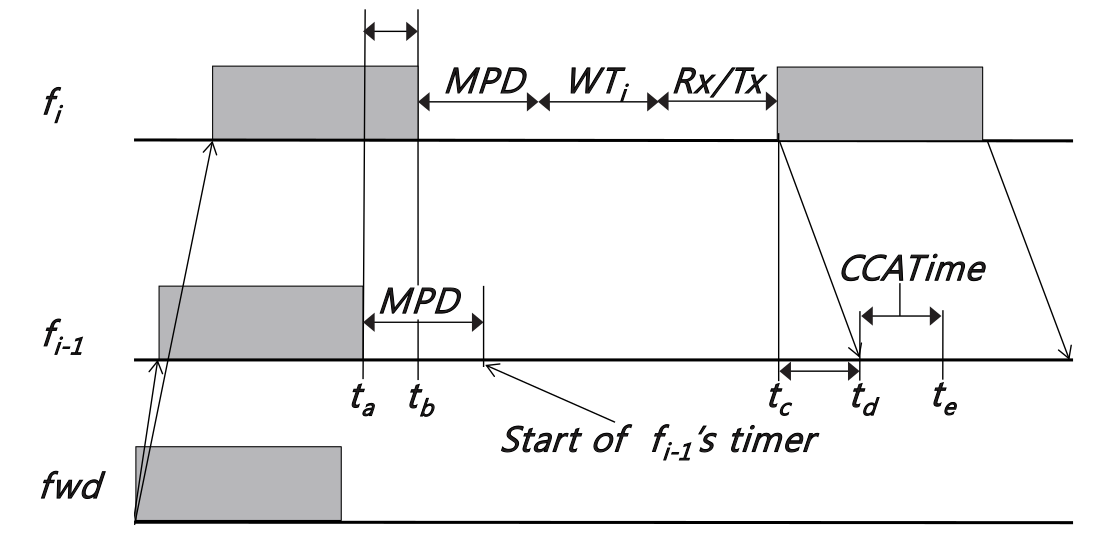
\includegraphics[width=\textwidth]{immagini/minDiff}
				\caption{Definition of $minDiff$ between $f_N$ and $f_{N-1}$ (\cite{6906275})}
				\label{fig:minDiff}
			\end{figure}
		
			\imgrefcap{fig:minDiff} depicts a situation where $fwd$ is the forwarder and $f_i$ (farther from fwd than $f_{i-1}$) relays the message before $f_{i-1}$. The two vehicles $f_i$ and $f_{i-1}$ complete receiving the message at different times ($t_a$ and $t_b$) due to propagation delay (calculated as $pd = d / s$, where $d$ is the distance between two points in space and $s$ is the wave propagation speed of the medium, i.e. $s=c$, the speed of light, in wireless communication). After reception we have additional amount of time in order to process and retransmit the message:
			\begin{itemize}
				\item Each PFC spends MAC Processing Delay (MPD) to process the message and then waits for $WT_i$ calculated according to whichever multi-hop algoritm is being used. As explained previously, this waiting time is inversely proportional to the distance between the PFC and $fwd$;
				\item After timer expiration, each PFC wait for Rx/Tx turnaround time ($Rx/Tx$), in order to switch their interface from reception to transmission mode.
			\end{itemize}
			After $f_i$ has forwarded the message, $f_{i-1}$ starts receiving it at $t_d$, $t_d-t_c$  being equal to $pd{f_{i-1}, f_i}$. The time between the PHY module of $f_{i-1}$ starts reception and the MAC module of the same vehicle is aware of reception is called $CCATime$. Hence, if $f_{i-1}$'s timer expires between $t_a$ and $t_e$, $f_{i-1}$'s transmission will collide with $f_i$'s. In order to accomplish succesful suppression, $f_{i-1}$'s timer should not expire  before $t_e$. 
			
			
			Given the fact that Propagation delay is not controllable and MPD, $Rx/Tx$ and $CCATime$ are usually standard-defined parameters, an algorithm can only manage the difference between waiting times of $f_i$ and $f_{i-1}$ (represented by $WT_i$ and $WT_{i-1}$ respectively in the following formula).
			To achieve succesful suppression, $f_{i-1}$ should wait until the forwarding from $f_i$ is detected by $f_{i-1}$ MAC layer, so $MPD+WT_{i-1}$ should be greater than $t_e - t_a$. Hence, $minDiff = (pd_{fwd, f_i} - pd_{fwd, f_{i-1}}) + pd_{f_i, f_{i-1}} + Rx/Tx + CCATime$.
		
		\subsection{Latency Analysis}
			\label{ssec:latency-analysis}
			The second problem ROFF tries to overcome is the effect of empty space in vehicle distribution on forwarding latency.
			
			The region where PFCs are placed can be defined as \textit{naive forwarding area} (NFA) and is defined as the intersection between:
			\begin{itemize}
				\item the transmission range of a forwarder $fwd$;
				\item the area in the opposite movement direction of the same forwarder $fwd$.
			\end{itemize}
			The distribution of vehicle inside NFA can vary in time; moreover, vehicles are not usually placed at the same distance, so empty spaces of various sizes exist inside the area.
			
			\begin{figure}[H]
				\centering
				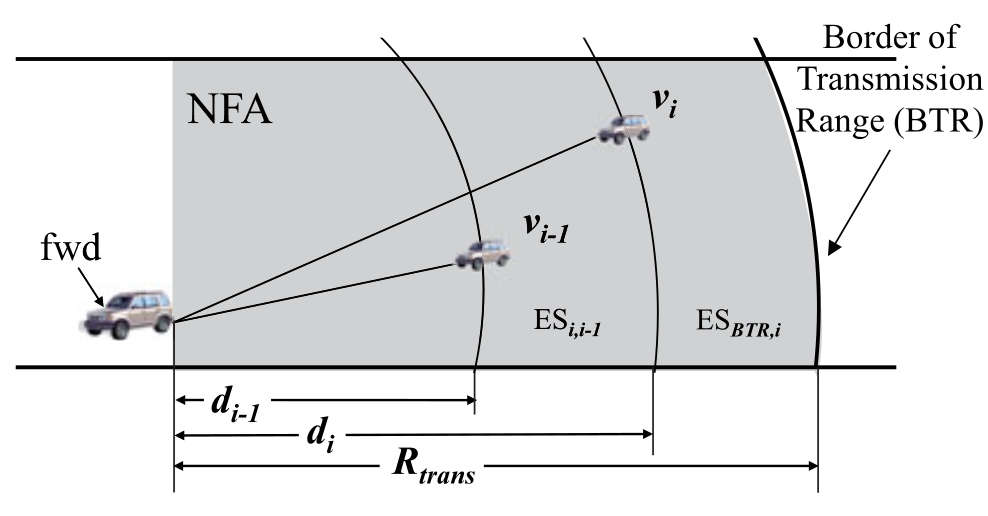
\includegraphics[width=\textwidth]{immagini/emptySpace}
				\caption{Definition of empty space (\cite{6906275})}
				\label{fig:emptySpace}
			\end{figure}
			
			Suppose that $S_v = \{v_i | 0 < i \leq M\}$ is a set of M vehicles inside NFA with vehicles ordered by distance between the vehicle and the previous forwarder in ascending order. Referring to Figure \ref{fig:emptySpace} , the empty space $ES_i,i-1$ between $v_i$ and $v_{i-1}$ is the segment within the two circles centered in $fwd$ with radius $d_{i-1}$ and $d_i$ respectively. Hence, the size of $ES_i,i-1$ is equal to $d_i - d{i-1}$.
			
			
			Large empty spaces have a negative effect on forwarding latency. There is no guarantee that the farthest vehicle from the previous forwarder become the FFC: lossy channel environments, shadowing and other phenomena can make any vehicle within NFA become the forwarder. Suppose that $fwd$ is the previous forwarder and there are two vehicles, $A$ and $B$, inside NFA where A is farther from $fwd$ than $B$, $A$ has not received the transmission from $fwd$ while B has. The empty space $ES_A,B$ between $A$ and $B$ influences the forwarding latency:
			\begin{itemize}
				\item if  $ES_A,B$ is small, $B$ relays the message after a short waiting time;
				\item if $ES_A,B$ is large, $B$ waits needlessly (since there is no other vehicle farther from $fwd$ which has received the message) a large amount of time.
			\end{itemize}
			ROFF aims at resolving the effect of empty spaces by allowing vehicles to choose waiting time inversely proportional to their \textit{unique forwarding priority} proportional to the distance between the vehicle and the previous forwarder, instead of using directly such distance in the waiting time computation.
		
	\section{ROFF Algorithm}
		The ROFF algorithm works under the following two assumptions:
		\begin{enumerate}
			\item each vehicle has access to a GPS system and a digital map;
			\item vehicles periodically (e.g. every 100 milliseconds) broadcast a Hello message containing various information, such as its position, velocity, etc. The period between each Hello message broadcast is called \textit{Beacon Interval}.
		\end{enumerate}
		The algorithm is composed of three components, as depicted in Figure \ref{fig:roffAlgo}.
	
		\begin{figure}[H]
			\centering
			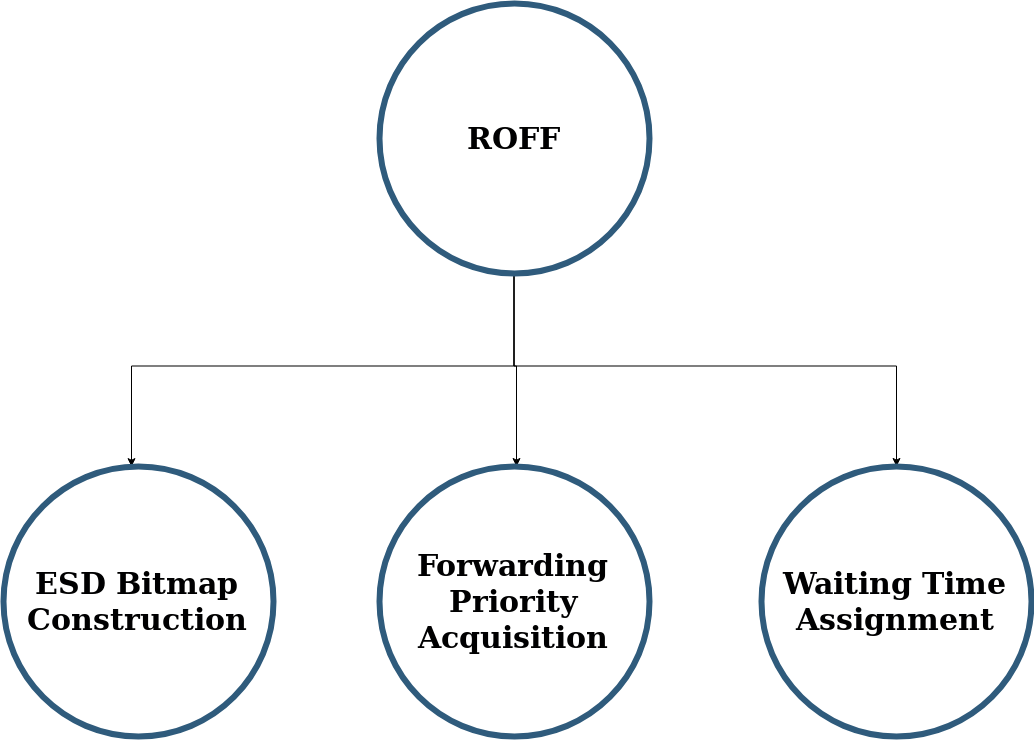
\includegraphics[width=0.7\textwidth]{immagini/roffAlgo}
			\caption{Components of ROFF algorithm}
			\label{fig:roffAlgo}
		\end{figure}
	
		The algorithm in short works as follows (additional information will be given in the following sections):
		\begin{itemize}
			\item when a forwarder relays an Alert Message, it also broadcasts a special structure called ESD Bitmap which describe the empty space distribution within the forwarderś NFA;
			\item PFCs which receive the Alert Message and the ESD Bitmap decide whether they are eligible for contention based on the ESD Bitmap;
			\item Eligible PFCs contend by choosing different waiting times based on a unique forwarding priority.
		\end{itemize}
	
		\subsection{ESD Bitmap Construction}
			Upon Hello Message reception, each vehicle uses the data within the message in order to update and maintain a structure called Neighbor Table (NBT) which monitors its local view (i.e. all the vehicles in the neighborhood of said vehicle). Each entry of the NBT contains:
			\begin{itemize}
				\item the ID of the neighbor;
				\item the position of the neighbor;
				\item the reception time of the Hello Message to verify the freshness of information and remove outdates entries.
			\end{itemize}
			An example of Neighbor Table of node with ID 0 is represented in Picture \ref{fig:nbt}.
				
			\begin{figure}[H]
				\centering
				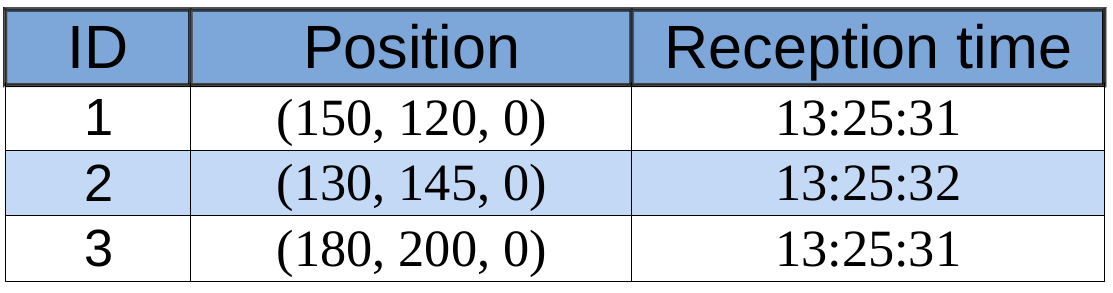
\includegraphics[width=0.7\textwidth]{immagini/nbt}
				\caption{Example of Neighbor Table of node with ID 0}
				\label{fig:nbt}
			\end{figure}
			Thanks to the NBT, the forwarder can advertise its neighborhood to other vehicles. We can define the set of neighbors detected by the forwarder as its \textit{local view}. If a vehicle who receives an Alert Message is not present inside the local view of the forwarder, then that vehicle cannot participate in contention.
			
			
			The NBT could be piggybacked as-is on the Alert Message, but the authors of ROFF identified some problems with this solution, such as the great overhead caused by the size of IDs. Hence, the proposed solution consists in compressing the NBT in a bitmap-like structure called ESD Bitmap. 
			
			
			In order to build the ESD Bitmap, first of all the forwarder measures the distance between itself and each of its neighbors listed in the NBT. Due to GPS granularity, distances are expressed at meter-level and can be represented with non-negative integers.
			
			\begin{figure}[H]
				\centering
				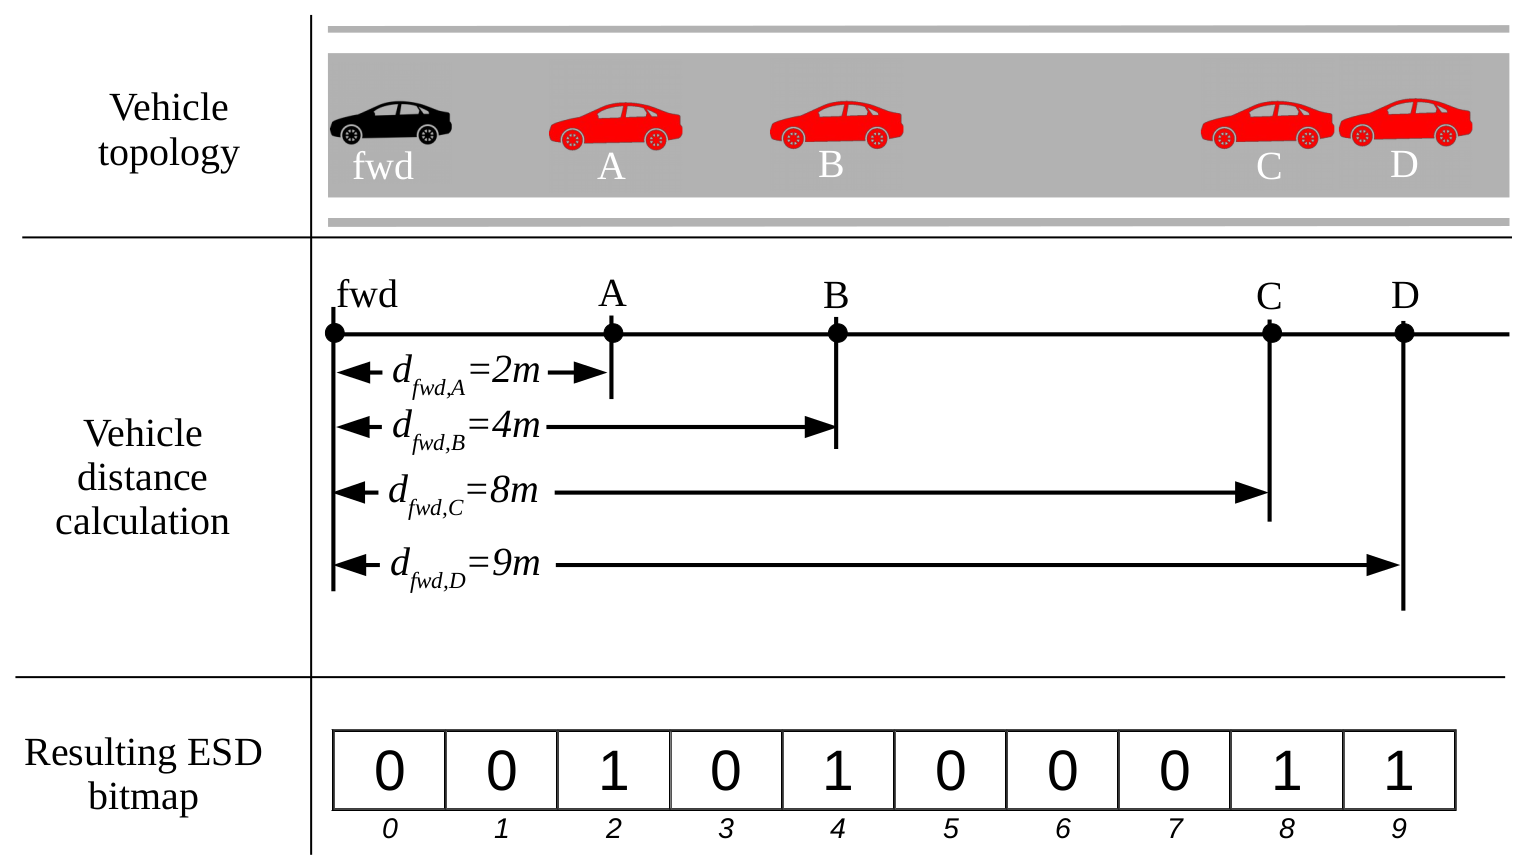
\includegraphics[width=\textwidth]{immagini/esdBitmapConstruction}
				\caption{ESD Bitmap construction with \textit{k} = 1}
				\label{fig:esdBitmapConstruction}
			\end{figure}
			
			After distance measurement, \textit{fwd} builds a bitmap to represent the measured distances by setting the \textit{i-th} bit to either:
			\begin{itemize}
				\item 1 if there is a PFC distant $d$ from \textit{fwd} such that $k * i \leq d \leq k * ( i + 1 ) - 1$;
				\item 0 otherwise.
			\end{itemize} 
			The parameter \textit{k}, called \textit{distance range}, identifies how many distances can be identified by the same bit in the ESD Bitmap. This parameter can be controlled to manage the compression level and the accuracy of the Bitmap. Increasing \textit{k} decreases the number of bits of the Bitmap, but every bit will identify \textit{k} different distances, hence losing precision.
			Picture \ref{fig:esdBitmapConstruction} shows the construction of an ESD Bitmap using $k = 1$.
			
			
			An ESD Bitmap using $k = 2$ is show in Figure \ref{fig:esdBitmapConstructionK2}. It is possible to see that the bit in position 4 represents distances $d$ such that $8 \leq d \leq 9$. 
			
			\begin{figure}[H]
				\centering
				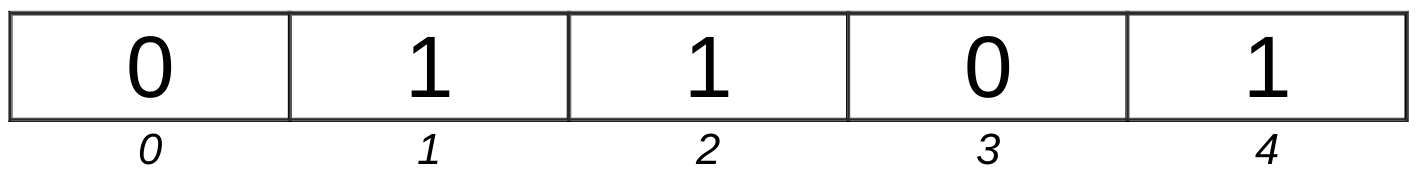
\includegraphics[width=\textwidth]{immagini/esdBitmapConstructionK2}
				\caption{Resulting ESD Bitmap with \textit{k} = 2}
				\label{fig:esdBitmapConstructionK2}
			\end{figure}
		
		\subsection{Forwarding Priority Acquisition}
			Whenever a PFC $f_i$ receives the Alert Message with included the ESD Bitmap from $fwd$, it checks whether the distance between itself and the previous forwarder is listed inside the bitmap (i.e. $f_i$ checks whether the bit in position $d(fwd, f_i)$ in the bitmap is equal to 1, assuming $k = 1$). If so, $f_i$ can participate in contention since it is inside the \textit{local view} of $fwd$. Otherwise, is cannot participate in contention to forward the Alert Message.
			
			
			After $f_i$ has entered contention, it can calculate its own forwarding priority based on the distances express by the ESD Bitmap. These distances are the distances of every other PFC which can participate in contention. Assuming that $L_{dist}$ is the list of distances ordered in ascending order and $distance = d(fwd, f_i)$, $f_i$'s forwarding priority is set as the rank of $distance$ inside $L_{dist}$. This way PFCs that are farther away from $fwd$ are assigned a higher forwarding priority, while PFCs nearer $fwd$ are assigned a lower forwarding priority.
			
			
			ROFF avoids assigning the same priority to two different PFCs by a technique called \textit{ID-based contention}. Using this technique, whenever a PFC $f_i$ receives an Alert Message it checks whether its NBT contains another vehicle $f_j$ whose distance from $fwd$ is the same as $f_i$'s (hence the distance is identified by the same bit in the bitmap). If so, $f_i$ participates in detection only if its ID is higher than the ID of $f_j$. In other words, if inside $f_i$'s NBT there exists an entry for $f_j$ such that $d(fwd, f_i) = d(fwd, f_j)$ and $ID_{f_j} > ID_{f_i}$, then $f_i$ defers its transmission. Figure \ref{fig:idBasedContention} depicts a scenario where node A does not participate in contention due to ID-based contention.
	
			\begin{figure}[H]
				\centering
				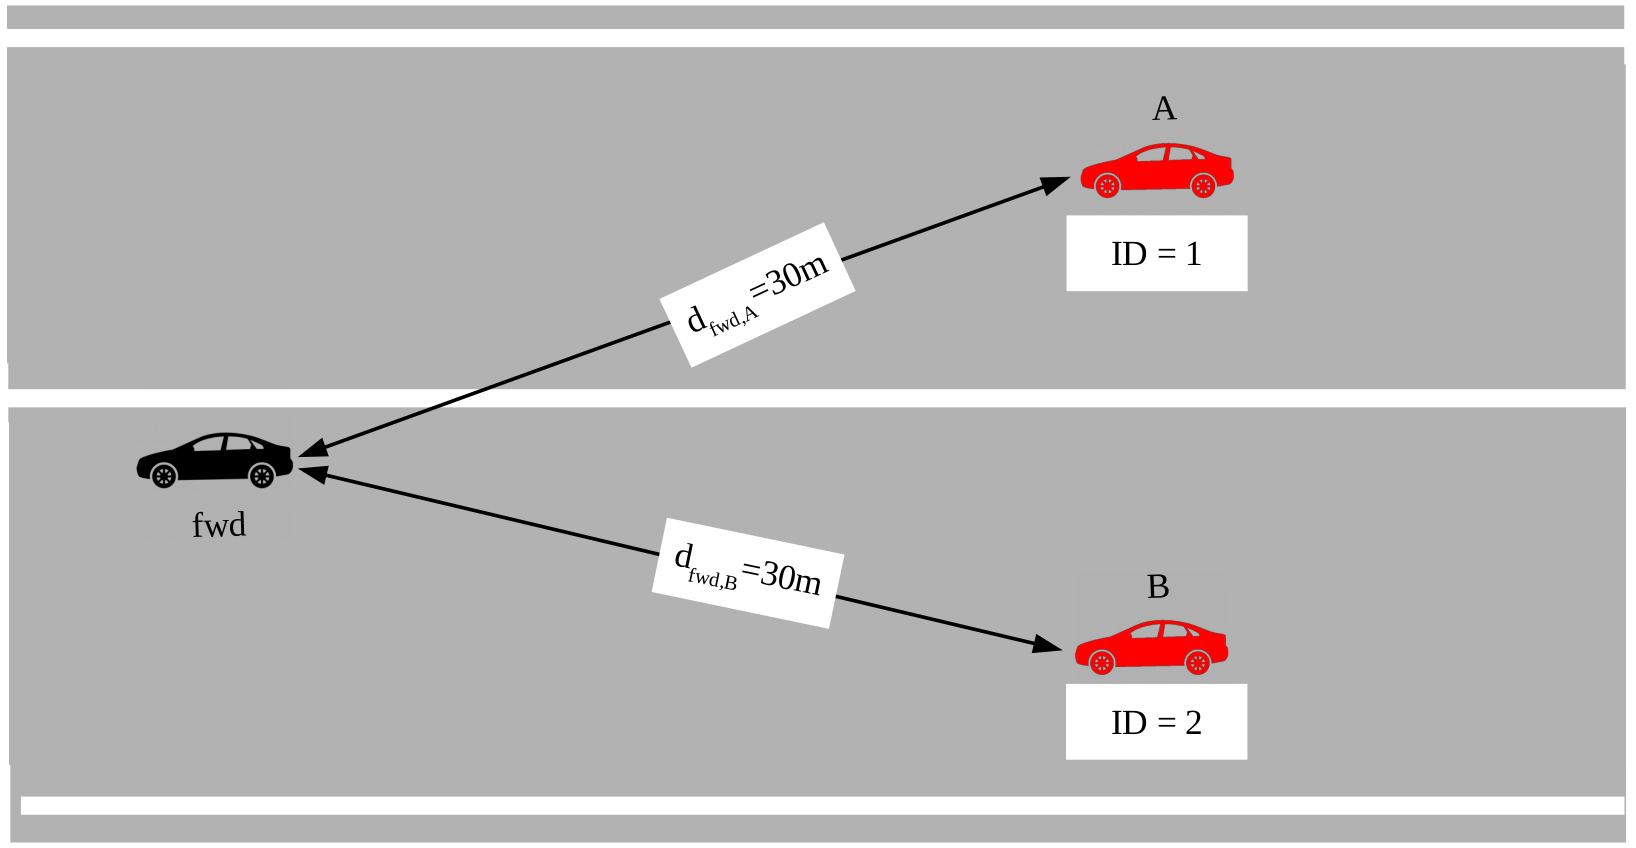
\includegraphics[width=\textwidth]{immagini/idBasedContention}
				\caption{ID-based contention: node A defers its transmission}
				\label{fig:idBasedContention}
			\end{figure}
		
		\section{Waiting Time Assignment}
			Once forwarding priorities are determined, ROFF assigns a waiting time that is inversely proportional to it. Letting $PFC(i)$ be the PFC with forwarding priority $i$ and $WT_p$ the waiting time of PFC $p$, in order to achieve successful suppression of transmission by $PFC(i-1)$, the waiting time of $PFC(i-1)$ should be at least longer by $minDiff_{PFC(i), PFC(i-1)}$ than waiting time of $PFC(i)$ (i.e. $WT_{PFC(i-1)} \geq WT_{PFC(i)} + minDiff_{PFC(i), PFC(i-1)})$. Hence, the waiting time of $PFC(k)$ is the sum of $minDiff$s between PFCs with forwarding priorities lower than $k$, as shown in Equation xxx. PFC with top priority (being equal to 1) broadcasts immediately and does not have to wait any time.
			
			$$WT_{PFC(k)} = \sum_{i=2}^{k} minDiff_{PFC(i),PFC(i-1)} (k \geq 2)$$
		
		
		
		
	